%%%%%%%%%%%%%%%%%%%%%%%%%%%%%%%%%%%%%%%%%%
\newpage
\subsection{Discussion of Study Findings}
\label{main-study:discussion:study}
%%%%%%%%%%%%%%%%%%%%%%%%%%%%%%%%%%%%%%%%%%
%%%%%%%%%%%%%%%%%%%%%%%%%%%%%%%%%%%%%%%%%%%%%%%%%%%%%%%%%%%%%%%%%%%%
% Present evidence -- and come up with possible interpretation/explanation,
% isn't this just theory generation?
%%%%%%%%%%%%%%%%%%%%%%%%%%%%%%%%%%%%%%%%%%%%%%%%%%%%%%%%%%%%%%%%%%%%
% NEED TO RELATE WITH OTHER PARTS OF CHAPTER: what are implications for other sections of the discussion, and also what are implications for design/further research in this area
%	\item RELATE TO METHODOGICAL RECOMMENDATIONS?
%	\item RELATE TO DESIGN:   (specific to WorkspaceMirror and general)
%	\item RELATE TO THEORY GEN
%%%%%%%%%%%%%%%%%%%%%%%%%%%%%%%%%%%%%%
% OTHER REPEATS FROM CHAPTER 4
%%%%%%%%%%%%%%%%%%%%%%%%%%%%%%%%%%%%%%

%%%%%%%%%%%%
% LEAD IN
%%%%%%%%%%%%
% \textbf{Chapters~\ref{chapter:exploratory_study}} and~\textbf{\ref{chapter:main_study}} reported a range of empirical results. This sections pulls together the findings from both chapters, and discusses their implications. \textit{THINK: focus on chapter 6?}
% This section discusses the findings from the study component of the field trial, 
%%%%%%%%%%%%%%%%%%%%%%%%%%%%%%%%%%%%%%%%%%%%%%%%%%%%%%%%%%%%%%%%%%%%%%%%%%%%%%%%%%%%%%%%%%%%%%%%%%%%%%%%
% Only a sample of the study findings. Need to justify the selection of these results.
% Most pertinent/interesting.  
%%%%%%%%%%%%%%%%%%%%%%%%%%%%%%%%%%%%%%%%%%%%%%%%%%%%%%%%%%%%%%%%%%%%%%%%%%%%%%%%%%%%%%%%%%%%%%%%%%%%%%%%
During the study, a broad range of data relating to PIM behaviour was collected over several months.  Whilst the exploratory study reported in \textbf{Chapter~\ref{chapter:exploratory_study}} was novel in terms of being a \textit{cross-tool} study, the study presented in this chapter is one of the few \textit{longitudinal} PIM studies carried out to date.  It is the only \textit{cross-tool}, \textit{longitudinal} study that the author is aware of. 
%%%%%%%%%%%%%%%%%%%%%%%%%%
% METH LIMITATIONS
%%%%%%%%%%%%%%%%%%%%%%%%%%
However, a number of methodological limitations are acknowledged.  These limit the generality of the results, and indicate possible directions for more follow-up work.  Firstly, like most other PIM studies, only a small number of participants took part.  In addition, the participants were all known to the author, and were technically experienced.  Ideally, similar studies should be carried out with more users from other backgrounds. However, such follow-up studies are outside the scope of this thesis.  % Key limitations in both components of the study are discussed in each section above  Methodological issues are discussed in depth in \textbf{Chapter~\ref{chapter:conclusion}}. 

%%%%%%%%%%%%%%%%%%%%%%%%%%%%%%%%%%%%%%%%%%%%%%%%%%%%%%%%%%%%%%%%%%%%%%%%%%%%%%%%%%%%%%%%%%%%%%%%%%%%%%
%%%%%%%%%%%%%%%%%%%%%%%%%%%%%%%%%%%%%%%%%%%%%%%%%%%%%%%%%%%%%%%%%%%%%%%%%%%%%%%%%%%%%%%%%%%%%%%%%%%%%%
%%%%%%%%%%%%%%%%%%%%%%%%%%%%%%%%%%%%%%%%%%%%%%%%%%%%%%%%%%%%%%%%%%%%%%%%%%%%%%%%%%%%%%%%%%%%%%%%%%%%%%
%%%%%%%%%%%%%%%%%%%%%%%%%%%%%%%%%%%%%%%%%%%%%%%%%%%%%%%%%%%%%%%%%%%%%%%%%%%%%%%%%%%%%%%%%%%%%%%%%%%%%%

%%%%%%%%%%%%%%%%%
% GROWTH
%%%%%%%%%%%%%%%%%
%%%%%%%%%%%%%%%%%%%%%%%%%%%%%%%%%%
\subsubsection{Longitudinal Insights into PIM behaviour}
\label{disc:study-discussion:growth}
%%%%%%%%%%%%%%%%%%%%%%%%%%%%%%%%%%
%\textbf{NEW: pressure/complexity/stress/never-ending}

%%%%%%%%%%%%%%%%%%%%%%%
% TO ADD SOMEWHERE?
%%%%%%%%%%%%%%%%%%%%%%%
%One consistent finding is that the personal information environments evolve slowly.  Even
%%%%%%%%%%%%%%%%%%%%%%%%%%%%%%%%%%%%%%%%%%%%%%%%%%%%%%%%%%%%%%%%%%%%%%%%%%%%%%%%%%%%%%%%%%
% Acquisition can be measured in terms of the turnover of items added to the collections.  Only approximate as deleted items not captured.  Item growth rates were broadly similar between files and email at about 5 per day.  However, note that the email growth rate does 
The study provided further insight into the four PIM sub-activities identified in the conceptual framework in \textbf{Chapter~\ref{chapter:bg}}.

Primarily, the growth of collections provided insight into the acquisition sub-activity.
% into how collections of personal information grow over time.
%%%%%%%%%%%%%%%%%%%%%%%%%%%
% NATURE OF COLLECTING
%%%%%%%%%%%%%%%%%%%%%%%%%%%
% Relative comparison: files and email much more intensive than bookmarks (possibly as bookmarks also stored in other tools, esp email?)
% Participants collected files, email and bookmarks incrementally over the course of the study -- incrementally adding to the respective collection. 
% For most participants, file and email collections both increased in size significantly over the course of the study.  Bookmark collections increased at a much lower rate.  
All participants actively collected files and email over the study.  In contrast, bookmarks were less actively collected, and increased in number at a much smaller rate (an average of 0.2 per day, compared to 4 per day for files). This ties in with the lack of importance of the bookmark collection reported by participants in the exploratory study.  However the idiosyncratic nature of PIM means that it is hard to generalize, since one participant, M4, collected them extensively.

%%%%%%%%%%%%%%%
% ACQUISITION -- Measure of turnover
%%%%%%%%%%%%%%
% Overall additions were most high in files and email, and less high in bookmarks.
% Acquisition was bursty.  Although not measured exactly here, 
The average figures suggest that items were added to the collections at a slow steady pace (in the two fastest-growing collections, files and email, approximately 5 items a day).  
However, it is argued here that acquisition was sporadic, and varied significantly over the course of the study.  Acquisition was marked by bursts corresponding to new pieces of work, and troughs corresponding to times away from the computer, e.g. holiday or using another computer.  An interesting direction for future work would be to track the increase in items per day, and correlate with the user's production activities.

%%%%%%%%%%%%%%%%%%%%%%%%%%%%%%%%%%%%%%%%%%%%%
% MORE TO ACQUISTION THAT FLAT INCREASE
%%%%%%%%%%%%%%%%%%%%%%%%%%%%%%%%%%%%%%%%%%%%%
Note that the figures presented reflect the net increase in items over the study (i.e. acquisitions minus deletions).  In particular, the email growth rate does not reflect the turnover in messages, including thousands of messages that were deleted and not kept.  It is argued that such a net figure is a better reflection of email growth, compared to the number that are downloaded. In email, acquisition over the long-term, is best conceptualized as acquisition minus deletion.

%%%%%%%%%%%%%%%%
% ORGANIZATION
%%%%%%%%%%%%%%%%
% Sparseness of organizational changes
% consider Impact on WM evaluation/PIM evaluation in general. Problems encountered for evaluation -- e.g. sparseness % add to methodological challenges for evaluation
% (ADD INCREMENTAL COUNT OF DELETED FOLDERS).
Growth rates were much lower for folders compared to items.  As organizing activity was relatively sparse, folder structures evolved slowly over the course of the study.  Even the participant who created the most folders, F2, only created 51 folders over the course of the study across all three tools.  Very few folder deletion and renaming events were observed over the study.  The two exceptions were F3 and M5 who deleted and moved a number of folders during one-off reorganizing episodes.  
This sparseness indicates the need to evaluate prototypes such as WM, which provide new organizing functionality, over the long-term.  % It is acknowledged that the sorting of items can be considered a form of ``retrieval-time organization''.  However, the study did not collect data on this aspect of organization, and focused purely on folder structures.

As can be seen from \textbf{Table~\ref{table:main-study:growth-rates-indiv}}, folder growth rates were higher in files relative to email and bookmarks for all but one participant.  The exception was F4 who carried out significant bookmark organization.  For the other participants, the higher folder growth in files reflects greater reliance on organizing in that collection.

% and were rarely reorganized.  
% any PIM-tool providing a new method of organizing material. Driven as production roles dictate. 
% \textit{Question -- would organizational changes also be as sparse for other forms of organization (e.g. sorting mechanisms for organizing on the fly)?}


%%%%%%%%%%%%%%%%
% MAINTENANCE
%%%%%%%%%%%%%%%%
%%%%%%%%%%%%%%%%%%
% Maintenance
%%%%%%%%%%%%%%%%%%
In all three tools, maintenance, e.g. archiving or deleting information, was performed rarely, if at all. In email, two participants archived large numbers of items (but no folders).  In bookmarks, no archiving was performed.  In files, two participants archived items and folders out of their collections: F3 to transfer information for working at home, and M5 due to a lack of space on his network drive.  In contrast, most participants, archived files (such as websites) \textit{into} their file collections.  This in-situ archiving runs counter to the traditional definition of archiving as the removal of items from a collection, e.g.~\citep{barreau:95}.   One interesting reason for not archiving material out of collections was that it made items harder to find at a later date.
% How often did users archive? How often did they delete?
% Highlight nature of archiving, based on observations in files (in-situ, incoming).
% However, large-scale maintenance happens rarely. Except for two participants who archived portions of their email collections, few items and folders were removed. 


%%%%%%%%%%%%%%%%
% RETRIEVAL
%%%%%%%%%%%%%%%%
%%%%%%%%%%%%%
% Retrieval
%%%%%%%%%%%%%
% Retrieval was clearly ongoing and is hards to capture data on. Perhaps a lab study is most appropriate to collect objective data on this short-term, repetitive aspect of PIM.  Or alternatively, more low-level measures but does this mean invasive logging, or qualitative self-reports.
No objective data was collected on the retrieval sub-activity.  Like the exploratory study, participants' qualitative feedback indicated that they relied on browsing and sorting, in preference to keyword search.  To collect objective data on retrieval practices, future research could potentially collect more detailed logs on one-off retrieval events.  However, such logging may be considered too invasive by participants.



%%%%%%%%%%%%%%%%%%%%%%%%%%%%%%%%%%%%%%%%%%%%%%%%%%%%%%%%%%%%%%%%%%%%%%%%
% Provides insight into the relative frequency of PIM sub-activities. 
% USE IN THEORY LATER
% Catch: limited to certain portions of the hierarchy.
%%%%%%%%%%%%%%%%%%%%%%%%%%%%%%%%%%%%%%%%%%%%%%%%%%%%%%%%%%%%%%%%%%%%%%%%
The data provides insight into the relative frequency of PIM sub-activities.  Acquisition, retrieval are ongoing but ``bursty'', as driven by the user's information needs.  Organization is more sporadic, and maintenance is very rare.  PIM can therefore be conceptualized as the process of incrementally adding items to a mass of older items, partially organized within a slowly evolving folder structure.  Many of the older items are archived in situ and rarely retrieved. However, as reported in \textbf{Chapter~\ref{chapter:exploratory_study}}, users still consider some of their older information to be highly important.

The relative frequency of PIM sub-activities contributes to the improved model of PIM developed in \textbf{Section~\ref{discussion:theoretical-framework}}.







%%%%%%%%%%%%%%%%%%%%%%%%%%%%%%%%%%%%%%%%%%%%%%%%%%%%%%%%%%%%%%%%%%
% OTHER ASPECTS
% speculate benefits of slow/ownership/pride/longevity
% but con of clutter
% Whilst some users suggested that they were proud of their data and liked having it around, others were clearly bothered by the clutter.
%%%%%%%%%%%%%%%%%%%%%%%%%%%%%%%%%%%%%%%%%%%%%%%%%%%%%%%%%%%%%%%%%%
% ongoing nature
% ITM MANAGEMENT - BUILD UP OVER TIME - FOLDER MANAGEMENT
% items need managing, then folders need managing - ongoing hell
%%%%%%%%%%%%%%%%%%%%%%%%%%%%%%%%%%%%%%%%%%%%%%%%%%%%%%%%%%%%%%%%%%

%%%%%%%%%%%%%%%%%%%%%%%%%%%%%%%%%%%%%%%%%%%%%%%%%%%%%%%%%%%%%%%%%%%%%%%%%%%%%%%%%%%%%%%%%%%%%%%%%%%%%%
%%%%%%%%%%%%%%%%%%%%%%%%%%%%%%%%%%%%%%%%%%%%%%%%%%%%%%%%%%%%%%%%%%%%%%%%%%%%%%%%%%%%%%%%%%%%%%%%%%%%%%
%%%%%%%%%%%%%%%%%%%%%%%%%%%%%%%%%%%%%%%%%%%%%%%%%%%%%%%%%%%%%%%%%%%%%%%%%%%%%%%%%%%%%%%%%%%%%%%%%%%%%%
%%%%%%%%%%%%%%%%%%%%%%%%%%%%%%%%%%%%%%%%%%%%%%%%%%%%%%%%%%%%%%%%%%%%%%%%%%%%%%%%%%%%%%%%%%%%%%%%%%%%%%

%%%%%%%%%%%%%%%%%%%%%%%%%%%%%%%%%%%%
\subsubsection{The Supporting Nature of PIM}
\label{disc:study-discussion:supporting}
%%%%%%%%%%%%%%%%%%%%%%%%%%%%%%%%%%%%

\textbf{Section~\ref{main-study:results:reflection}} presented a range of qualitative comments from participants which highlighted the background nature of PIM.  PIM was seen as an activity they performed every day to support their research, administrative, and educational roles.  However, it was also seen to be of low priority, and in some cases as a distraction, or as a ``break from real work''.
%%%%%%%%%%%%%%%%
% PARADOX PIM
%%%%%%%%%%%%%%%%
% The supporting nature of PIM is highlighted by the following quote from participant M6 in the main study reported in : . Similar paradoxical views were reported by several participants in the study: that PIM is a necessary activity, but one that is equally unimportant.
This indicates a paradoxical situation, whereby participants were driven to manage their information, yet ran the risk of wasting time in doing so.
% When asked how their time could be better spent, participants typically responded that they should be doing ``real work'' rather than managing files or email.
Indeed the \textit{discretionary} nature of PIM means that users can choose whether to perform it or not, and if they do, to what extent they perform it.
% Participant F2 identified ``writing papers'' as what he should be doing rather than managing files.
% PIM was often seem as an escape or a therapeutic break from work.
% Yet users are clearly driven to carry out PIM in some form on a regular basis, if as nothing more than a break from ``real work''. % ADD QUOTE.

%%%%%%%%%%%%%%%%%%%%%%
% LACK OF REFLECTION
%%%%%%%%%%%%%%%%%%%%%%
% Lack of reflection - emphasised background nature of PIM.
% lack of reflection (how tool and study in general prompted reflection).  
The study also highlighted the \textit{lack of attention} many users devote to PIM.  Although they carried out PIM everyday, PIM was not an activity that many participants reported spending time focused on.
%%%%%%%%%%%%%%%%%%%%%%%%%%%%%%%
% PROMOTION OF REFLECTION
%%%%%%%%%%%%%%%%%%%%%%%%%%%%%%%
% Participants suggested that both the study and tool interventions increased
% the amount of time they devoted to reflecting on PIM. 
% \textit{Self-auditing effect:	Need to delete that, that's where that is}
Most participants in the main study indicated that their participation, combined with the design intervention, lead them to devote more attention to PIM. % he interviews had a clear ``self-auditing'' effect.

%%%%%%%%%%%%%%%%%%%%%%%%%%%%%%%%%%%%%%%%%%%%%%%%
% ARGUE THAT PIM IS SUPPORTING BASED ON THIS
% Instead users are focused on production goals.  
%%%%%%%%%%%%%%%%%%%%%%%%%%%%%%%%%%%%%%%%%%%%%%%%
These results support the conceptualization of PIM as a \textit{supporting} activity.  This theme is developed further in \textbf{Section~\ref{discussion:theoretical-framework}}, where it is suggested that it is user's high-level production activities and goals, their ``real work'', that provide direction to their otherwise discretionary PIM activities.
%not the prime reason that people use their computers.
% The conceptualization of PIM as a supporting activity is discussed in greater detail in .



%%%%%%%%%%%%%%%%%%%%%%%%%%%%%%%%%%%%%%%%%%%%%%%%%%%%%%%%%%%%%%%%%%%%%%%%%%%%%%%%%%%%%%%%%%%%%%%%%%%%%%
%%%%%%%%%%%%%%%%%%%%%%%%%%%%%%%%%%%%%%%%%%%%%%%%%%%%%%%%%%%%%%%%%%%%%%%%%%%%%%%%%%%%%%%%%%%%%%%%%%%%%%
%%%%%%%%%%%%%%%%%%%%%%%%%%%%%%%%%%%%%%%%%%%%%%%%%%%%%%%%%%%%%%%%%%%%%%%%%%%%%%%%%%%%%%%%%%%%%%%%%%%%%%
%%%%%%%%%%%%%%%%%%%%%%%%%%%%%%%%%%%%%%%%%%%%%%%%%%%%%%%%%%%%%%%%%%%%%%%%%%%%%%%%%%%%%%%%%%%%%%%%%%%%%%

%%%%%%%%%%%%%%%%%
% Changes
%%%%%%%%%%%%%%%%%
%%%%%%%%%%%%%%%%%%%%%%%%%%%%%%%%%%%%
\subsubsection{Changes in Organizing Strategy}
\label{disc:study-discussion:changes}
%%%%%%%%%%%%%%%%%%%%%%%%%%%%%%%%%%%%
% PIM changes tended to be incremental and subtle, reflecting peoples' PIM strategies.  This findings is used to argue for modifications to the model of PIM changes proposed by~\citet{ob:97}.

%%%%%%%%%%%%%%%%%%%%%%%%%%%%%
% subtle c c c c c changes
%%%%%%%%%%%%%%%%%%%%%%%%%%%%%
% We did not observe any ``global'' changes in strategy along the lines of those discussed by~\citet{ob:97}
% Slow and piecemeal, incremental. It is noted that changes were relatively minor
% as illustrated by the findings presented in \textbf{Section~\ref{main-study:results:changes}}, and discussed in \textbf{Section~\ref{main-study:discussion:study}}. 
Two of the eight participants made significant changes to their PIM strategies over the course of the field study: % Two participants made significant changes as follows:
\begin{itemize}

% worked on working information, few aspects, in certain tools (certain stuff?)
\item Participant F3 changed the way that he managed his active files, moving many from ``My Documents'' to the ``Desktop'' and creating a number of new folders to organize them.

\item Participant M5 made two changes.  Firstly, he changed how he managed old information in both files and email -- moving all old project data under an ``Old'' folder in each collection.  Secondly, he reported filing more email by the end of the study.  In particular, he described how he was filing more messages relating to conference paper submissions.
% -- possibly driven by the demands of a new production activity taken up by the user in question.
% : one activity example. What about re-org of stuff into old? (actually managing working stuff in the same way)
\end{itemize}



%%%%%%%%%%%%%%%%%%%%%%%%%
% CHANGES WERE SUBTLE
%%%%%%%%%%%%%%%%%%%%%%%%%
% The observed changes were more incremental than those observed by B�lter. 
% The observed changes corresponded to small shifts in overall strategy.  Typically the change was highly targeted at how a specific type of information was managed.  
% Participants differed in the relative proportions of the low-level strategies employed. 
The study provided examples of the changes which may occur in user's management strategies over time. However, the changes observed were \textit{incremental} rather than the \textit{global}, wholesale shifts discussed in~\citet{ob:97}, e.g. \textit{no-filer} to \textit{spring-cleaner}. In other words, the changes amounted to subtle changes in the participant's overall PIM practices, equivalent to adaptations in low-level organizing strategy for certain types of information.   
%%%%%%%%%%%%%%%%%%%%%%%%%%%%%%%%%%%%
% LINK TO MODEL IN NEXT SECTION
%%%%%%%%%%%%%%%%%%%%%%%%%%%%%%%%%%%%
The next section, extends the model of strategy changes from~\citet{ob:97} to reflect these observations.

%%%%%%%%%%%%%%%%%%%%%%%%%%%%%%%%%%%%
% Although subtle, still useful
%%%%%%%%%%%%%%%%%%%%%%%%%%%%%%%%%%%%
For both participants, the changes, though subtle, were worthwhile: M5: \textit{``the [email] folders that I've created, they only take up 2\% or 4\% [of the inbox]. [Does that make a difference?] Yes, because most of the stuff that comes in is day-to-day stuff I deal with today, the things I extract now are things with a longer due time''}.


%%%%%%%%%%%%%%%%%%%%%%%%%
% All pro-organizing
%%%%%%%%%%%%%%%%%%%%%%%%%
The changes observed over the field study were all \textit{pro-organizing} (involving increases in organizing effort).  No study participants were observed changing in favour of being less organized, although some had reported such changes from before the study. Note that although participant F1 abandoned his existing bookmark folders on starting a new job, he started building up a new collection using similar filing strategies as before. % Relate to earlier substantial historical changes were reported, including both increases and decreases in organizing tendency

%%%%%%%%%%%%%%%%%
% DISCUSS MODEL WHY BIG SHIFTS ARE HARD: 
%%%%%%%%%%%%%%%%%
% Huge amount of work in changing everything.  Easier to change one little thing
% argue in favour of incremental design?
% the supporting nature of PIM means that 
As discussed in \textbf{Section~\ref{main-study:results:reflection}}, many users devote little time to planning and executing changes in strategy.  Thus it makes sense that only subtle shifts in strategy were observed. As participant M8 commented, there is a huge amount of effort involved in a major reorganization or change in strategy.  His feedback emphasised that such ``grand shifts'' are time-consuming and non-trivial.   Instead, it is much easier to make small adjustments.  Of course, substantial changes in overall trait may occur, but these would happen at major life points and it is not surprising that none were encountered during the study.


%%%%%%%%%%%%%%%%%%%%%%%%%%%%%%%%%%%%%%%%%%%%%%%%
% IMPACT ON EVAL
%%%%%%%%%%%%%%%%%%%%%%%%%%%%%%%%%%%%%%%%%%%%%%%%
% As strategies can take a long time to evolve, it may take time for users to adapt to new PIM-tools.
The observed changes emphasise the need to evaluate PIM designs over the long-term, since designs which depend upon a change in strategy may take time to be adopted.  In terms of WM, the incremental nature of the observed changes may be a partial explanation for the slow uptake of WM.  
% Despite the incremental action of WM, a
As indicated by participant M8, the change in strategy to make use of mirrored folders may be substantial.


% These findings regarding changes are used in a number of ways later in this chapter.
%%%%%%%%%%%%%%%%%%%%%%%%%%%%%%%%%%%%%%%%%%%%%%%%%%%%%%%%%%%%%%%%%%%%%%%%%%%%%
% USE IN EVAL DISC: TO EXPLAIN SUCCESS OF WM, slow change, partial change
%%%%%%%%%%%%%%%%%%%%%%%%%%%%%%%%%%%%%%%%%%%%%%%%%%%%%%%%%%%%%%%%%%%%%%%%%%%%%

%The slow rate of changes in PIM strategy may act as an inhibiting factor in the uptake of new tools.  A new tool offering a new form of organization required a huge amount of effort on the part of the user to adopt. Therefore it is envisaged that folder-mirroring functionality should be optional.





%%%%%%%%%%%%%%%%%%%%%%%%%%%%%%%%%%%%%%%%%%%%%%%%%%
\subsubsection{Factors influencing the Changes}
%%%%%%%%%%%%%%%%%%%%%%%%%%%%%%%%%%%%%%%%%%%%%%%%%%

%%%%%%%%%%
% FACTORS
%%%%%%%%%%
%  the two participants who made the most significant strategy changes did not
A number of factors were noted that influenced the changes in strategy.  Firstly, participation in the study clearly had an effect on the study changes.  Both \textit{changers} stated that increased reflection on PIM due to the study was the main factor causing the changes.  
%%%%%%%%%%%%%%%%%%%%%%%%%%%%%%%%%%%%%%
% Would changes have happened anyway? - without the intervention?
%%%%%%%%%%%%%%%%%%%%%%%%%%%%%%%%%%%%%%
It should be considered whether the changes would have happened anyway without the study intervention.  Participant M5 stated that he had been planning the changes for some time but had not implemented them due to the perceived effort involved.  He stated that the guided tour during phase 1 involved carrying out much of the effort (assessing folders on a case by case basis).  Thus, the amount of effort left to reorganize his folder structures was much lower.  Such influence is an unavoidable effect of a field trial -- the experimenter will always have some influence on what users are doing.  Not carrying out face-to-face interviews may be one route to lessening such effects. % eads to possible future work based on a less intrusive study.  However, then there may be privacy implications, since the intrusion did at least remind the participants that they were being tracked.

%%%%%%%%%%%%%%%%%%%%%%%%%%%%%%%%%%%%%%%%%%%%%%%%%%%
% Effects of study much greater than tool
%%%%%%%%%%%%%%%%%%%%%%%%%%%%%%%%%%%%%%%%%%%%%%%%%%%
% Acknowledge relative influence of study and tool on changes. The influences of both design intervention and study participation on changes in user strategy are discussed
Secondly, the author's design intervention also impacted PIM behaviour.  However, against the author's expectations, neither changer considered WM to be a major contributory factor, even though both performed some mirroring over the course of the study.  M5 stated that the prompting increased his reflection on PIM but to a lesser degree than the interviews.  The author had anticipated that WM would stimulate pro-organizing strategy changes by allowing users to leverage filing investment in one collection across to other collections.  However, this was not the case -- the participants who used it extensively, employed WM in support of their existing filing strategies, and did not report filing more than they had done previously. % Of the \textit{non-changers}, two (F2 and F4) made extensive use of WM, using it mirror an average of 14 folder creations events, mostly between files and email.  These participants 

Finally, Participant F3 also noted a social pressure to be more organized, \textit{``I mean I really am envious of people like X who has all his folders worked out. He is really organized''}.





%%%%%%%%%%%%%%%%%%%%%%%%%%%%%%%%%%%%%%%%%%%%%%%%%%%%%%%%%%%%%%%%%%%%%%%%%%%%%%%%%%%%%%%%%%%%%%%%%%%%%%
%%%%%%%%%%%%%%%%%%%%%%%%%%%%%%%%%%%%%%%%%%%%%%%%%%%%%%%%%%%%%%%%%%%%%%%%%%%%%%%%%%%%%%%%%%%%%%%%%%%%%%
%%%%%%%%%%%%%%%%%%%%%%%%%%%%%%%%%%%%%%%%%%%%%%%%%%%%%%%%%%%%%%%%%%%%%%%%%%%%%%%%%%%%%%%%%%%%%%%%%%%%%%
%%%%%%%%%%%%%%%%%%%%%%%%%%%%%%%%%%%%%%%%%%%%%%%%%%%%%%%%%%%%%%%%%%%%%%%%%%%%%%%%%%%%%%%%%%%%%%%%%%%%%%
%%%%%%%%%%%%%%%%%%%%%%%%%%%%%%%%%%%%
\subsubsection{Towards a Model of Changes in Organizing Strategy}
\label{main-study:discussion:changes-model}
%%%%%%%%%%%%%%%%%%%%%%%%%%%%%%%%%%%%
%%%%%%%%%%%%%%%%%%%%%%%
% EXTEND THE MODEL
%%%%%%%%%%%%%%%%%%%%%%%
% This section offers a new conceptualization of PIM strategies.  Firstly, \textbf{Section~\ref{discussion:strategies-cross-tool}} develops a cross-tool model of PIM strategy, drawing from the cross-tool perspective developed in \textbf{Section~\ref{discussion:cross-tool}}.
% In addition, strategies may change over time.  They are not pre-determined, but may evolve.  Empirical data of real-life PIM strategies was presented in \textbf{Chapter~\ref{chapter:main-study}}.
% Building on the observation of multiple strategies in \textbf{Chapter~\ref{chapter:exploratory_study}}, this section develops a new model of PIM strategy changes is proposed, 

%%%%%%%%%%%%%%%%%%%%%%%%%%%%%%%%%%%%%%%%%%%%%%%%%%%%%%%%%%%%%%%%%%%%%%%
% Build on Balter
% LINK TO THEORY DEV:BALTER: (towards improved model of changes in PIM strategies)
% (influencing factors are discussed). 
% Balter's study is based on an abstract classification, and the corners of his model represent overall extreme traits. Instead, what changes is the RATIO of information that is dealt with in a particular way
%%%%%%%%%%%%%%%%%%%%%%%%%%%%%%%%%%%%%%%%%%%%%%%%%%%%%%%%%%%%%%%%%%%%%%%
A model of changes in email organizing strategy was proposed in~\citet{ob:97}.  Firstly, this can be criticised for focusing on unrealistic user traits such as \textit{frequent filer} and \textit{spring cleaner}.  \textbf{Section~\ref{exp-study:discussion:multiple-strategies}} argued that such classifications are inaccurate as they portray abstract, extreme user traits.  % replace chapter with section
%%%%%%%%%%%%%%%%%%%%%%%%%%%%%%%%%%
% Multiple strategies revisited}
%%%%%%%%%%%%%%%%%%%%%%%%%%%%%%%%%%
% USE: relate to multiple strategies data 
% MS confirms ES: users again employ a range of strategies (EXPLORATORY CONFIRMATION). 
% /variegated/multi-faceted
% : one user - multiple strategies depending on type of information being managed
Secondly, the model can be criticised for portraying strategy changes as major shifts.  
In this section, B�lter's model is extended to account for the observations of \textit{incremental} changes made in this chapter.  % As in B�lter's work, a focus is taken on changes within specific tools only.
% Based on the observations outlined above, B�lter's model of user strategy changes is extended to reflect the incremental strategy changes that were observed.  
As in B�lter's work, a focus is taken on \textit{email}, but the model can be also applied to other tool contexts\footnote{Note that different changes may happen simultaneously in different tools, as each represents an independent PIM sub-system.  For example, a user may abandon her bookmarks, but start filing her email more carefully. However this is beyond the scope of the model proposed here.}.

%%%%%%%%%%%%%%%%%%%%%%%%%%%%%%%%%%%
% REVISIT THE MODEL FROM CH 4
%%%%%%%%%%%%%%%%%%%%%%%%%%%%%%%%%%%
The model draws on the multiple strategies model from \textbf{Section~\ref{exp-study:discussion:multiple-strategies}} in which a user's tool-specific organizing strategy can be represented as the relative percentages of low-level strategies employed.  If one assumes two low-level strategies (\textit{frequent filing} and \textit{spring cleaning}), the multiple strategy can be plotted on a graph, where each axis indicates the relative proportions of new messages that are organized with each strategy.
%%%%%%%%%%%%%
% CHANGES IN THIS MODEL AND SCENARIO CODENAME JOE
%%%%%%%%%%%%%
An incremental change can therefore be represented as a \textit{shift in the relative proportions of information managed with a particular strategy}.  \textbf{Figure~\ref{fig:discussion:new-change-model}} provides two example changes based on the life of an example fictional user, Joe.  Joe starts with an overall multiple strategy of 10\% frequent filing and 90\% spring cleaning, indicated on the graph with a star. The two changes are as follows:
\begin{itemize}

\item \textit{Scenario 1: Joe starts e-dating with Mary} -- In the early stages of this intense relationship, Joe receives a large number of messages from her. He files all of Mary's messages immediately within a ``Mary'' folder as they mean so much to him.  Thus the overall percentage of email that is frequently filed increases to 12\%, resulting in a \textit{pro-organizing} shift.  This reflects the larger percentage of emails which are being organized immediately. % EXPLAIN WHY ORGANIZING STRATIGHT AWAY IS MORE PRO-ORGANIZING

\item \textit{Scenario 2: Joe starts going out with Mary in the real world} -- The second change happens when Joe starts spending all his time with Mary. Due to the demands on his time, he has less time to read email, let alone to file messages.  The relative proportion of email being immediately filed goes down.  Joe still files, but starts to rely on spring-cleaning messages.  This is an example of a \textit{organizing-neutral} shift.  

\end{itemize}

%%%%%%%%%%%%%%%%%%%%%%%%%%%%%%%%%%%%%%
% %%%%%%%%%%%%%%%%%%%%%%%%%%%%%%%%%%%%
% FIGURE - A new model of changes in PIM strategy
% %%%%%%%%%%%%%%%%%%%%%%%%%%%%%%%%%%%%
%%%%%%%%%%%%%%%%%%%%%%%%%%%%%%%%%%%%%%
\begin{figure}[hbtp]
	\begin{center}
		\leavevmode
		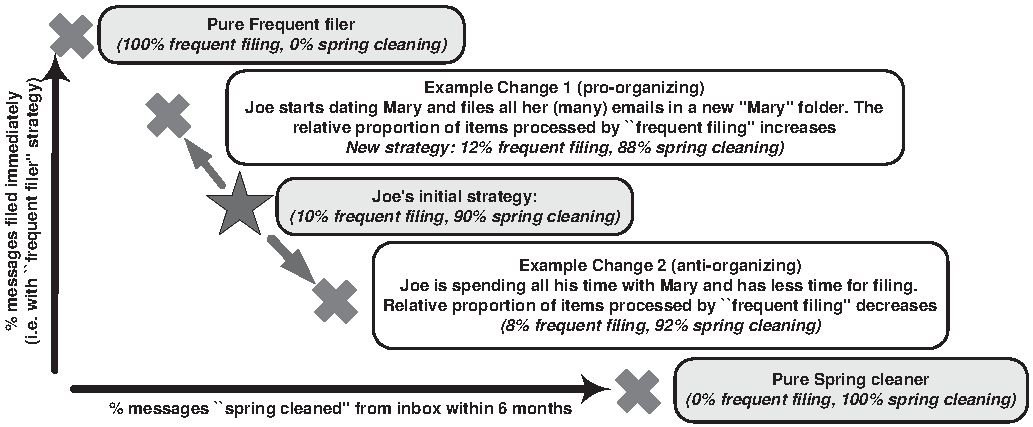
\includegraphics[width=\textwidth]{pictures/main-study/new-change-model.pdf}
	\end{center}
	\caption{A model of incremental changes in email organizing strategy}
	\label{fig:discussion:new-change-model}
\end{figure}
% CONSIDER: extending model to show both major shifts and minor shifts.}
% ADD: real examples from our study data

%%%%%%%%%%%%%%%%%%
% LIMITATIONS
%%%%%%%%%%%%%%%%%
A number of simplifying assumptions are acknowledged.  A first assumption is that all messages are filed at some point, via frequent filing or spring-cleaning.  A more realistic model would be multi-dimensional to account for other strategies, e.g. the non-filing of some messages.  Secondly, the model does not capture changes in how items are organized with a particular strategy.  For example, participant M5 moved many older project folders into a top-level `old' folder.  This does not represent a shift between strategies, but an adjustment to information that has already been filed.  Despite these simplifications, it is argued that the model provides a more realistic portrayal of changes in organizing strategy, and emphasises their incremental nature.  
% This section offers a new conceptualization of PIM strategies.  Firstly, \textbf{Section~\ref{discussion:strategies-cross-tool}} develops a cross-tool model of PIM strategy, drawing from the cross-tool perspective developed in \textbf{Section~\ref{discussion:cross-tool}}.
Furthermore, the model indicates the potential for developing improved conceptualizations of PIM strategies, and how they change over time.

% But note still abstracts the low-level manner of filing employed etc.

%%%%%%%%%%%%%%%%%%%%%%%%%%%%%%%%%%%%%%%%%%%%%%%%%%
% STUDY EXAMPLES: link changes with multiple strategies. 
%%%%%%%%%%%%%%%%%%%%%%%%%%%%%%%%%%%%%%%%%%%%%%%%%%
% In particular, it is suggested that small changes are made as demanded by new production activities and types of information.
% RELATE TO MULIPLE STRATEGIES The change data observed in the main study corresponds with the observation of \textit{multiple strategies} outlined in \textbf{Chapter~\ref{chapter:exploratory_study}}.  Multiple strategies were identified in the context of specific tools, as well as across multiple tools for most participants.

%%%%%%%%%%%%%%%%%%%%%%%%%%%%%%%%%%%%%%%%%%%%%%%%%%%%%%%%%%%%%%%%%%%%%%%%%%%%%%%%%%%%%%%%%%%%%%%%%%%%%%%%%%%%%%%%%
%%%%%%%%%%%%%%%%%%%%%%%%%%%%%%%%%%%%%%%%%%%%%%%%%%%%%%%%%%%%%%%%%%%%%%%%%%%%%%%%%%%%%%%%%%%%%%%%%%%%%%%%%%%%%%%%%
%%%%%%%%%%%%%%%%%%%%%%%%%%%%%%%%%%%%%%%%%%%%%%%%%%%%%%%%%%%%%%%%%%%%%%%%%%%%%%%%%%%%%%%%%%%%%%%%%%%%%%%%%%%%%%%%%
%%%%%%%%%%%%%%%%%%%%%%%%%%%%%%%%%%%%%%%%%%%%%%%%%%%%%%%%%%%%%%%%%%%%%%%%%%%%%%%%%%%%%%%%%%%%%%%%%%%%%%%%%%%%%%%%%

%%%%%%%%%%%%%%%%%%%%%%%%
% \subsubsection{Summary}
%%%%%%%%%%%%%%%%%%%%%%%%
%%%%%%%%%%%%%%%%%%%%%%%%%%
\subsubsection{Summary}
%%%%%%%%%%%%%%%%%%%%%%%%%%

%%%%%%%%%%%%%%%%%%%%%%%%%%%%%%%%%%
% AIM 2: FURTHER STUDY
%%%%%%%%%%%%%%%%%%%%%%%%%%%%%%%%%%
This section has discussed a number of the findings from the study component of the field trial.  Firstly, growth rates were compared between the three collections, along with the relative frequencies of the different PIM sub-activities.  The study highlighted the supporting property of PIM, and the lack of reflection on the part of users. 
The study also provided data on a number of real-life adaptations of PIM strategy.  A simple model of incremental strategy changes was proposed.
% This section highlighted the incremental nature of the observed strategy changes, and based on this data, outlined an extension to B�lter's model of strategy changes~\citep{ob:97}.   

%%%%%%%%%%%%%%%%%%%%%%%%%%%%%%%%%%%%%%%%%%%%
% MOVING ON: Towards Deeper Insights}
% Set the scene for the discussion chapter,  ...
%%%%%%%%%%%%%%%%%%%%%%%%%%%%%%%%%%%%%%%%%%%%
% \textbf{Section~\ref{main-study:discussion}} discussed the findings presented in this chapter in the context of the prior stages of this programme of research, as well as the previous work reported in \textbf{Chapter~\ref{chapter:review}}. 
Next, \textbf{Chapter~\ref{chapter:discussion}} moves on to combine the findings from this chapter with those from the wider thesis.


%%%%%%%%%%%%%%%%%%%%%%%%%%
% \subsubsection{Summary}
%%%%%%%%%%%%%%%%%%%%%%%%%%
% The study findings are used to explain design results in the next section, develop design recommendations in \textbf{Section X}, and theory in \textbf{Section Y}. % think about order ...
% This section considered longitudinal insights from the study.  These findings are used in further discussion in \textbf{Chapter~\ref{chapter:discussion}}.  

%%%%%%%%%%%%%%%%%%%%%%%%%%%%%%%%
% END: DISCUSSION - CHANGES
%%%%%%%%%%%%%%%%%%%%%%%%%%%%%%%%

%%%%%%%%%
% FIN
%%%%%%%%%
